\documentclass[12pt, a4paper]{report}

% --- Typography & Encoding ---
\usepackage[T1]{fontenc}
\usepackage[utf8]{inputenc}
\usepackage{newtxtext,newtxmath} % Times New Roman-like typography
\usepackage{microtype}
\usepackage{setspace}
\onehalfspacing

% --- Page Geometry ---
\usepackage[
  a4paper,
  left=1.00in,
  right=0.85in,
  top=0.78in,
  bottom=0.80in,
  headheight=16pt,
  headsep=8pt,
  footskip=28pt
]{geometry}

% --- Custom Chapter/Section Formats ---
\usepackage{titlesec}
\titleformat{\chapter}[hang]
  {\bfseries\fontsize{16}{19}\selectfont}
  {\thechapter.}{0.55em}{\MakeUppercase}
\titlespacing*{\chapter}{0pt}{0pt}{20pt}

\titleformat{\section}
  {\bfseries\fontsize{13}{16}\selectfont}
  {\thesection.}{0.55em}{}
\titlespacing*{\section}{0pt}{16pt}{8pt}

\titleformat{\subsection}
  {\bfseries\fontsize{12}{15}\selectfont}
  {\thesubsection.}{0.55em}{}
\titlespacing*{\subsection}{0pt}{14pt}{6pt}

% Simplify chapter headers to remove "Chapter" prefix
\makeatletter
\renewcommand{\@makechapterhead}[1]{%
  \vspace*{0pt}%
  {\parindent\z@ \raggedright \normalfont
    \bfseries\fontsize{16}{19}\selectfont
    \thechapter.\quad\MakeUppercase{#1}\par\nobreak
    \vskip 20pt}}
\makeatother

% --- Page Borders (MACE Style) ---
\usepackage{tikz}
\usepackage{eso-pic}
\AddToShipoutPictureBG{%
\begin{tikzpicture}[remember picture,overlay]
\draw[line width=1.0pt]
    ([xshift=0.3in,yshift=-0.3in]current page.north west)
    rectangle
    ([xshift=-0.3in,yshift=0.3in]current page.south east);
\end{tikzpicture}%
}

% --- Header and Footer (User Request) ---
\usepackage{fancyhdr}
\newcommand{\ReportTitle}{ClauseIQ -- Machine Learning-Based Contract Clause Classification and Intelligent Search System}
\newcommand{\DepartmentName}{Department of Computer Applications, MACE}

\pagestyle{fancy}
\fancyhf{}
\fancyhead[R]{\small\ReportTitle}
\fancyfoot[L]{\small\DepartmentName}
\fancyfoot[R]{\small\thepage}
\renewcommand{\headrulewidth}{0.6pt}
\renewcommand{\footrulewidth}{0.6pt}

% Apply same style on chapter-opening pages
\fancypagestyle{plain}{%
  \fancyhf{}
  \fancyhead[R]{\small\ReportTitle}
  \fancyfoot[L]{\small\DepartmentName}
  \fancyfoot[R]{\small\thepage}
  \renewcommand{\headrulewidth}{0.6pt}
  \renewcommand{\footrulewidth}{0.6pt}
}

% --- Paragraph Formatting ---
\setlength{\parindent}{0pt}
\setlength{\parskip}{0.75em}
\usepackage{ragged2e}
\AtBeginDocument{\justifying}

% --- Code Snippet Styling ---
\usepackage{xcolor}
\usepackage{listings}
\definecolor{codebg}{gray}{0.14}
\definecolor{codetext}{gray}{0.96}
\lstset{
  basicstyle=\ttfamily\small\color{codetext},
  backgroundcolor=\color{codebg},
  frame=single,
  rulecolor=\color{codebg},
  breaklines=true,
  columns=fullflexible,
  keepspaces=true,
  showstringspaces=false,
  xleftmargin=0.04\textwidth,
  xrightmargin=0.04\textwidth,
  aboveskip=8pt,
  belowskip=4pt
}

% --- Mathematics, Lists, Tables ---
\usepackage{amsmath, amssymb}
\usepackage{booktabs}
\usepackage{array}
\usepackage{longtable}
\usepackage{tabularx}
\usepackage{enumitem}
\setlist[itemize]{leftmargin=1.5em,itemsep=2pt,topsep=4pt}
\setlist[enumerate]{leftmargin=1.7em,itemsep=2pt,topsep=4pt}

% --- Hyperlinks & References ---
\usepackage[hidelinks]{hyperref}
\usepackage{xurl}

\begin{document}

% ==========================================
% CHAPTER 1: INTRODUCTION
% ==========================================
\chapter{INTRODUCTION}
\label{ch:introduction}

\section{Contract Review Problems in Industries}
Commercial contracts represent the legal and operational backbone of virtually all corporate business transactions. These documents, which include Non-Disclosure Agreements (NDAs), Service Level Agreements (SLAs), Master Service Agreements (MSAs), joint venture structures, and licensing arrangements, outline the rights, duties, and liabilities of the contracting parties. However, despite their critical importance, the administration and evaluation of these documents remain heavily dependent on manual processes in corporate environments. 

Organizations routinely manage thousands of active agreements. As transaction volumes grow, purely manual review does not scale, creating major challenges:
\begin{itemize}
    \item \textbf{Cognitive Fatigue and Errors:} Legal documents are dense, lengthy, and written in highly specialized legal prose. Manual review of hundreds of pages of text causes cognitive fatigue among lawyers, leading to oversight of critical clauses, financial obligations, or non-compliance risks.
    \item \textbf{Inconsistent Interpretations:} Different manual reviewers may interpret identical or similar clauses differently, leading to inconsistent compliance metrics across organization boundaries.
    \item \textbf{High Operational Cost and Bottlenecks:} Due diligence audits and contract reviews require hours of expensive legal labor. The resulting bottlenecks can delay sales cycles and procurement processes.
\end{itemize}

\section{Why Manual Clause Searching is Difficult}
When legal teams or business executives need to locate specific provisions (such as indemnity limits, termination notice periods, or governing law clauses) across historical documents, they face significant hurdles. Manual searching is highly challenging for several key reasons:
\begin{itemize}
    \item \textbf{Lack of Semantic Capabilities:} Standard keyword searches (e.g., using Ctrl+F) look for exact string matches. Legal concepts, however, can be drafted using various synonyms. For example, a search for ``Liability Limit'' will miss clauses titled ``Limitation of Liability'' or sentences referring to ``indemnification caps'' or ``maximum aggregate exposure.''
    \item \textbf{Structural Variation:} Contracts are unstructured text files without a standard schema. Some documents embed key clauses within sections on general covenants, while others isolate them in dedicated appendices.
    \item \textbf{Document Formats:} Legacy contracts are frequently stored as scanned PDFs or image-based files without extractable text layers, necessitating manual page-by-page review.
\end{itemize}

\section{Importance of Legal NLP}
Legal Natural Language Processing (Legal NLP) is a specialized branch of artificial intelligence that focuses on analyzing, processing, and understanding legal documents. Unlike generic NLP systems trained on news articles or social media, Legal NLP addresses the unique characteristics of legal text:
\begin{itemize}
    \item \textbf{Syntactic Complexity:} Legal drafting features extremely long sentences, nested clauses, parenthetical explanations, and archaic vocabulary (often referred to as ``legalese''). Legal NLP tools are optimized to parse these complex syntax trees.
    \item \textbf{Semantic Precision:} In the legal domain, minor phrasing variations can alter a party's rights or obligations. Legal NLP systems use contextual representations to capture subtle semantic details that generic models overlook.
    \item \textbf{Contextual Disambiguation:} Words like ``consideration,'' ``performance,'' or ``execution'' have specific meanings in legal contexts that differ from their everyday usage. Legal NLP models resolve these ambiguities using surrounding context.
\end{itemize}

\section{Importance of Machine Learning}
Machine Learning (ML) acts as the driving engine behind automated document classification and search. By representing text numerically (vectorization), ML models learn patterns from training data to classify new, unseen texts. Instead of relying on manual rules or regular expressions, which fail when encountering variations in drafting, machine learning models learn representation boundaries. This enables automated classification of clauses with high generalization capabilities, reducing the manual review workload from days to seconds.

\section{Why Classical Machine Learning is Chosen instead of Deep Learning or RAG}
While deep learning models (such as BERT, RoBERTa, or LSTM) and Large Language Models (LLMs) used in Retrieval-Augmented Generation (RAG) have become popular in general NLP, classical machine learning remains the preferred choice for this project. The selection is justified by several practical and technical factors:
\begin{enumerate}
    \item \textbf{Interpretability and Transparency:} In legal applications, explainability is crucial. Lawyers must understand why a system classified a clause under a specific category. Classical ML algorithms like Logistic Regression and Naive Bayes provide clear coefficients and probabilities, and Random Forests output feature importances. In contrast, deep neural networks and LLMs function as black boxes, making error tracing highly difficult.
    \item \textbf{Computational Efficiency and Low Resource Footprint:} LLMs and deep learning models require expensive, high-end Graphical Processing Units (GPUs) for training and inference, which translates to high operational costs. Classical ML algorithms (such as Naive Bayes, Logistic Regression, Linear SVM, and Random Forests) are highly lightweight, enabling fast training and sub-millisecond inference on standard CPUs. This makes local desktop deployment viable and cost-effective.
    \item \textbf{Determinism and Prevention of Hallucination:} Generative AI models and RAG pipelines are prone to hallucinating facts, misinterpreting legal limits, or outputting text that does not exist in the source document. In legal compliance, a single hallucination can lead to significant liability. Classical ML models perform deterministic classification based strictly on the vocabulary present in the source text, eliminating the risk of hallucination.
    \item \textbf{Fit Within MCA Mini Project Scope:} Developing and optimizing deep learning models or setting up complex RAG orchestrations requires massive datasets, lengthy training times, and expensive APIs. Classical machine learning combined with Term Frequency-Inverse Document Frequency (TF-IDF) feature matrices is appropriate for the time constraints and academic scope of an MCA Mini Project. It demonstrates core machine learning principles—data preprocessing, feature extraction, classifier training, comparison, and evaluation—without unnecessary complexity.
\end{enumerate}

\section{Project Transition: From DocuMind AI to ClauseIQ}
The project was initially proposed under the title \textbf{DocuMind AI}. The initial concept was designed to build a general-purpose document intelligence system that could process multiple file types (PDFs, Word documents, images, and text files) across various domains (financial invoices, medical records, and legal files). 

However, during the initial feasibility study, this broad scope was found to be impractical within the time constraints of the MCA Mini Project. Trying to cover diverse document domains would result in shallow models and poor accuracy due to conflicting vocabularies. 

Consequently, the project scope was refined and focused exclusively on the legal domain under the new title \textbf{ClauseIQ}. ClauseIQ focuses on legal contracts, concentrating on automated clause extraction, 41-category classification, and intelligent similarity-based search. This narrowed focus allows for deep optimization of features and algorithms, leveraging domain-specific legal vocabularies to deliver high accuracy. A more ambitious deep-learning / RAG-based system (originally proposed as "DocuMind AI") was considered but was found to be too broad for this stage and has been deferred to a possible fourth-semester main project.

\section{Introduction to the CUAD Dataset}
ClauseIQ utilizes the \textbf{Contract Understanding Atticus Dataset (CUAD)}, developed by The Atticus Project. CUAD is a curated, expert-annotated corpus specifically designed for legal contract clause classification. It contains over 13,000 legal clauses extracted from 510 commercial contracts drawn from the U.S. Securities and Exchange Commission's public EDGAR database and expert-annotated by lawyers and law students associated with The Atticus Project. CUAD identifies 41 categories of clauses that are routinely reviewed in corporate transactions — such as Governing Law, Termination for Convenience, Non-Compete, and Cap on Liability — spanning more than 13,000 individually annotated clause instances. This makes it one of the largest, highest-quality, expert-labelled legal NLP resources publicly available, and a natural fit for a supervised clause-classification task.

\section{Two Key Objectives of ClauseIQ}
The ClauseIQ system is designed to achieve two primary functional objectives:
\begin{enumerate}
    \item \textbf{Contract Clause Classification:} Given the text of a clause (or a labelled span extracted from a contract), predict which of the 41 CUAD categories it belongs to, so that a reviewer can be automatically shown ``this looks like a Non-Compete clause'' instead of reading the whole document.
    \item \textbf{Intelligent Clause Search:} Given a natural-language query (e.g. ``find clauses that cap our liability''), retrieve the most relevant clauses across the corpus using TF-IDF vector representations and cosine similarity, without requiring an exact keyword match.
\end{enumerate}

Together, classification and search form a lightweight ``contract intelligence'' pipeline that mirrors, at a much smaller scale, the kind of tooling used in commercial contract-review products.

\section{Project Scope}
The scope of ClauseIQ includes:
\begin{itemize}
    \item Developing a preprocessing pipeline to clean raw contract texts.
    \item Implementing feature extraction using TF-IDF vectorization with unigrams and bigrams.
    \item Training and evaluating four classical machine learning classifiers: Multinomial Naive Bayes, Support Vector Machine (Linear SVM), Logistic Regression, and Random Forest.
    \item Developing a search module using Cosine Similarity to find relevant clauses.
    \item Providing a user-friendly interface to upload contracts, view classified clauses, and perform search queries.
\end{itemize}
This initial report documents the first phase of the project: dataset finalisation, supporting literature review, exploratory data analysis, preprocessing design, algorithm selection, project pipeline, and feasibility analysis. Model training, evaluation and deployment are addressed in the subsequent implementation sprints and reported in the final report.

\section{Project Objectives}
The core engineering objectives are:
\begin{itemize}
    \item To automate the tedious process of manual contract review.
    \item To achieve high classification accuracy and Macro F1-scores across all 41 categories in the CUAD dataset.
    \item To minimize query latency in the similarity search module.
    \item To build an explainable system that presents classification probabilities.
\end{itemize}

\section{Report Organization}
This initial report is organized into three main chapters. Chapter 1 provides the introduction, background, importance of Legal NLP, algorithmic choices, project transition, and objectives. Chapter 2 reviews the supporting literature, summarizing three relevant IEEE publications, followed by a comparative analysis and justification of the design decisions. Chapter 3 contains the System Analysis, detailing the CUAD dataset, preprocessing steps, algorithm workflows, pseudo-codes, and project pipeline.

\newpage

% ==========================================
% CHAPTER 2: SUPPORTING LITERATURE
% ==========================================
\chapter{SUPPORTING LITERATURE}
\label{ch:supporting_literature}

\section{Paper 1 -- Legal Natural Language Processing From 2015 to 2022: A Comprehensive Systematic Mapping Study of Advances and Applications}
\label{sec:paper1}

Authors: Quevedo Caballero E., Černý T., Rodriguez A., Rivas P., Yero J., Sooksatra K., Taibi D. (2024)\\
Title: ``Legal Natural Language Processing From 2015 to 2022: A Comprehensive Systematic Mapping Study of Advances and Applications.''\\
Journal: \textit{IEEE Access}, vol. 12, pp. 145286--145317.\\
DOI: \url{https://doi.org/10.1109/ACCESS.2024.3414967}

\paragraph{Area of Work:}
The paper presents a systematic mapping study that maps the literature, research trends, and advances in Legal NLP from 2015 to 2022, providing both quantitative statistics and qualitative categorizations.

\paragraph{Dataset:}
The research utilized a search protocol across four indexers, identifying 536 initial papers and filtering them to select 75 primary publications for in-depth analysis.

\paragraph{Methodology:}
The authors conducted a Systematic Mapping Study (SMS) to categorize primary publications based on research problems, publication venues, tasks, and methodologies, identifying research gaps and establishing a baseline for the field.

\paragraph{Algorithms:}
The review covers various algorithmic paradigms including rule-based architectures, traditional machine learning models, and deep learning or transformer architectures applied to legal tasks.

\paragraph{Results:}
The paper maps the distribution of Legal NLP research, identifying multiclass classification, summarization, and question answering as the primary task domains. It quantitatively highlights key open challenges in the field, including the lack of curated datasets, specialized ontology designs, and accessibility issues.

\paragraph{Advantages:}
Provides a comprehensive baseline that maps out the evolution of Legal NLP, helping researchers identify active subfields and under-explored areas.

\paragraph{Future Scope:}
Recommends establishing standard benchmark datasets for diverse legal tasks, building domain-specific legal ontologies, and investigating privacy-preserving architectures.

\begin{table}[h]
\centering
\small
\begin{tabular}{p{3.5cm}p{11.5cm}}
\toprule
Parameter & Details \\
\hline
Title & Legal Natural Language Processing From 2015 to 2022: A Systematic Mapping Study \\
Area of Work & Systematic mapping of Legal NLP applications and advancements \\
Dataset & Survey of 536 initial studies, filtering down to 75 primary publications \\
Methodology & PRISMA-style mapping, descriptive statistics, and research problem categorization \\
Algorithms & Traditional statistical models, machine learning, and transformer architectures \\
Results & Mapped core tasks (classification, QA); identified dataset scarcity and ontology gaps \\
Advantages & Comprehensive overview of the state of the art; highlights research trends \\
Future Scope & Creation of curated datasets, domain-specific ontologies, and privacy architectures \\
\bottomrule
\end{tabular}
\caption{Summary of Paper 1}
\label{tab:paper1_summary}
\end{table}

\newpage

\section{Paper 2 -- Exploring LLMs Applications in Law: A Literature Review on Current Legal NLP Approaches}
\label{sec:paper2}

Authors: Siino M., Falco M., Croce D., Rosso P. (2025)\\
Title: ``Exploring LLMs Applications in Law: A Literature Review on Current Legal NLP Approaches.''\\
Journal: \textit{IEEE Access}, vol. 13, pp. 18253--18276.\\
DOI: \url{https://doi.org/10.1109/ACCESS.2025.3533217}

\paragraph{Area of Work:}
This paper is a systematic literature review mapping the recent integration of transformer-based NLP and Large Language Models (LLMs) across legal tasks.

\paragraph{Dataset:}
The study systematically reviewed 61 selected publications published between 2017 and 2023, analyzing benchmarks like CUAD and ContractNLI.

\paragraph{Methodology:}
The authors followed a systematic database search and snowballing review process to select relevant articles, categorizing them into application domains and analyzing model configurations and evaluation metrics.

\paragraph{Algorithms:}
The review covers transformer models (BERT, RoBERTa, Legal-BERT, CaseBERT, T5) and generative GPT architectures.

\paragraph{Results:}
The paper maps the upsurge of LLM research across domains like document analysis, case prediction, and contract review. It confirms that fine-tuning models on domain-specific corpora (e.g., Legal-BERT) consistently yields better results than generic baselines, while identifying gaps in model hallucination, privacy, and computational costs.

\paragraph{Advantages:}
Provides a structured overview of modern transformer/LLM applications in law, highlighting the limits of generative AI in high-liability fields.

\paragraph{Future Scope:}
Focuses on prompt engineering techniques, federated learning for privacy preservation, and hybrid architectures combining LLMs with symbolic reasoning.

\begin{table}[h]
\centering
\small
\begin{tabular}{p{3.5cm}p{11.5cm}}
\toprule
Parameter & Details \\
\hline
Title & Exploring LLMs Applications in Law: A Literature Review \\
Area of Work & Systematic literature review of Transformer and LLM applications in law \\
Dataset & Survey of 61 core publications (utilizing CUAD, ContractNLI, etc.) \\
Methodology & PRISMA-style database search, snowballing, and taxonomic categorization \\
Algorithms & BERT, RoBERTa, Legal-BERT, CaseBERT, T5, and GPT architectures \\
Results & Confirmed performance gains of domain-specific fine-tuning; mapped legal application domains \\
Advantages & Identifies critical open research challenges like hallucinations and high costs \\
Future Scope & Prompt engineering, federated learning, and hybrid symbolic architectures \\
\bottomrule
\end{tabular}
\caption{Summary of Paper 2}
\label{tab:paper2_summary}
\end{table}

\newpage

\section{Paper 3 -- Named Entity Recognition Utilized to Enhance Text Classification While Preserving Privacy}
\label{sec:paper3}

Authors: Kutbi M. (2023)\\
Title: ``Named Entity Recognition Utilized to Enhance Text Classification While Preserving Privacy.''\\
Journal: \textit{IEEE Access}, vol. 11, pp. 117576--117581.\\
DOI: \url{https://doi.org/10.1109/ACCESS.2023.3325895}

\paragraph{Area of Work:}
The paper investigates privacy-preserving text classification, focusing on using Named Entity Recognition (NER) as an enhancement preprocessing step.

\paragraph{Dataset:}
Evaluated on standard text classification benchmarks and an in-house collected legal document dataset.

\paragraph{Methodology:}
The author proposes identifying sensitive entities (such as names, dates, organizations, and locations) using NER and replacing them with generic entity labels. The modified text is then converted into TF-IDF representation and passed to classical classifiers.

\paragraph{Algorithms:}
Evaluated using Naive Bayes, Support Vector Machines (SVM), Decision Tree Induction, and Nearest Neighbor classifiers.

\paragraph{Results:}
Experimental results showed that incorporating NER-based entity replacement achieved high accuracy (above 95\%) and strong F1-scores. The approach successfully reduces vocabulary dimensionality and preserves privacy without degrading the classification performance of downstream models.

\paragraph{Advantages:}
Provides an effective, simple preprocessing method that handles sensitive legal text, protecting privacy while maintaining high classifier accuracy.

\paragraph{Future Scope:}
Exploring deep learning-based NER and zero-shot domain adaptation to improve entity replacement robustness in unstructured texts.

\begin{table}[h]
\centering
\small
\begin{tabular}{p{3.5cm}p{11.5cm}}
\toprule
Parameter & Details \\
\hline
Title & Named Entity Recognition Utilized to Enhance Text Classification While Preserving Privacy \\
Area of Work & Privacy-preserving text classification using NER preprocessing \\
Dataset & Standard text classification benchmarks and an in-house legal document dataset \\
Methodology & NER-based entity detection and replacement, feature extraction, and classification \\
Algorithms & Naive Bayes, Support Vector Machines (SVM), Decision Trees, and Nearest Neighbor \\
Results & Achieved accuracy above 95\%; successfully reduced dimensionality and preserved privacy \\
Advantages & Protects sensitive data while maintaining downstream classifier accuracy \\
Future Scope & Integration of deep learning NER models and zero-shot domain adaptation \\
\bottomrule
\end{tabular}
\caption{Summary of Paper 3}
\label{tab:paper3_summary}
\end{table}

\newpage

\section{Literature Review Summary}
\label{sec:lit_review_summary}

\begin{table}[h]
\centering
\small
\begin{tabular}{p{3.0cm}p{4.2cm}p{4.2cm}p{3.8cm}}
\toprule
Paper & Main Focus & Key Finding & Relevance to ClauseIQ \\
\hline
Quevedo Caballero et al. (2024) & Systematic mapping of Legal NLP research (2015--2022) & Identified rapid research growth, task categories, and dataset/ontology gaps & Establishes clause classification as a valid task and supports CUAD selection \\
\hline
Siino et al. (2025) & Systematic review of Transformer and LLM applications in law & Confirms domain-specific fine-tuning outperforms generic models; notes cost/privacy limits & Contextualizes ClauseIQ and highlights the practical need for cost-efficient models \\
\hline
Kutbi (2023) & Privacy-preserving text classification using NER preprocessing & NER tag replacement reduces features and preserves privacy while achieving >95\% accuracy & Justifies classical classifiers (NB, SVM) and guides privacy-friendly preprocessing \\
\bottomrule
\end{tabular}
\caption{Literature Review Comparison Table}
\label{tab:literature_summary}
\end{table}

\section{Findings and Proposals}
\label{sec:findings_and_proposals}
The reviewed literature converges on three key points that directly shape ClauseIQ's design. First, contract clause classification and semantic clause search are recognized, well-motivated sub-tasks within Legal NLP, as mapped out in the systematic reviews of both Quevedo Caballero et al. (2024) and Siino et al. (2025), and CUAD is an established, high-quality benchmark for evaluating them. Second, literature shows that combining feature extraction with classification is highly effective for legal texts; specifically, Kutbi (2023) demonstrates that incorporating feature engineering steps (like identifying named entities) can significantly support downstream classifiers such as Naive Bayes and Support Vector Machines, achieving accuracies above 95\%. Third, because legal clause classification datasets like CUAD are heavily imbalanced, classical machine learning classifiers (Logistic Regression, Naive Bayes, SVM, and Random Forest) serve as highly interpretable and resource-efficient models for the task. The literature confirms that domain-specific features and structured preprocessing are essential to handle high-dimensional, sparse text distributions.

Based on these findings from the literature, ClauseIQ proposes a lightweight, interpretable, and computationally efficient classical Machine Learning pipeline. First, legal text classification is established as a valid and critical Legal NLP task, for which the expert-annotated Contract Understanding Atticus Dataset (CUAD) serves as an appropriate and rigorous benchmark. To extract features from raw contract text, TF-IDF vectorization (utilizing both unigram and bigram representations) is proposed to build an interpretable, length-normalized feature matrix. On this feature space, four classical classifiers---namely Multinomial Naive Bayes, Support Vector Machines (SVM), Logistic Regression, and Random Forest---will be systematically trained and compared to classify clauses into the 41 CUAD categories. Furthermore, the system will leverage cosine similarity over these TF-IDF vector representations to support intelligent clause search and retrieve relevant provisions based on natural language queries. Initially, the project focuses strictly on this classical pipeline, ensuring high interpretability and CPU-friendly execution, while deferring computationally intensive deep learning and transformer-based architectures to potential future extensions.


\newpage

% ==========================================
% CHAPTER 3: SYSTEM ANALYSIS
% ==========================================
\chapter{SYSTEM ANALYSIS}
\label{ch:system_analysis}

All figures, statistics and code outputs in this section were produced by actually loading and analysing the real CUAD v1 dataset (obtained from the official Atticus Project GitHub repository, \url{https://github.com/TheAtticusProject/cuad}) rather than a simulated or placeholder dataset.

\section{Analysis of the Dataset}

\subsection{About the Dataset}
The Contract Understanding Atticus Dataset (CUAD) v1 is sourced from the Atticus Project and distributed at \url{https://github.com/TheAtticusProject/cuad} (and mirrored on Hugging Face Datasets). It contains 510 real commercial contracts collected from the U.S. Securities and Exchange Commission's public EDGAR filing system, spanning 25 contract types (Distributor Agreements, Franchise Agreements, Licence Agreements, Strategic Alliance Agreements, etc.). Each contract has been manually annotated by law-student and attorney annotators against 41 clause categories that lawyers routinely review during due diligence — for example Governing Law, Anti-Assignment, Cap On Liability, Non-Compete, and Ip Ownership Assignment. In its raw distributed form, CUAD is released as a SQuAD-style question-answering JSON file (\texttt{CUADv1.json}), where each of the 41 categories is phrased as a ``question'' (e.g. ``Highlight the parts of this contract related to ‘Non-Compete’...'') and the answer is one or more text spans (the actual clause text) located inside the contract.

For ClauseIQ's classification and search use case, this QA-style format was converted into a flat, clause-level table: each row is one annotated clause span, together with the contract it came from and its category label. This conversion was performed directly on the official \texttt{CUADv1.json} file using a Python script (\texttt{json} + \texttt{pandas}), producing the working dataset \texttt{clauseiq\_dataset.csv} used for all analysis in this report.
\begin{itemize}
    \item \textbf{Dataset source:} \url{https://github.com/TheAtticusProject/cuad}
    \item \textbf{Raw file used:} \texttt{CUADv1.json} (SQuAD-style question-answering format)
    \item \textbf{Contracts:} 510 real commercial contracts sourced from SEC EDGAR
    \item \textbf{Clause categories (classes):} 41
    \item \textbf{Annotated clause spans after flattening and de-duplication:} 13,823
    \item \textbf{License:} Creative Commons Attribution 4.0 (CC BY 4.0)
\end{itemize}

\subsection{Explore the Dataset}
The flattened clause-level dataset was loaded with pandas and inspected using the same exploratory workflow used for structured tabular data: shape, data types, first records, missing values and summary statistics.

\paragraph{a) Shape and data types}
The database contains 13,823 rows and 5 columns:
\begin{table}[h]
\centering
\small
\begin{tabular}{p{4cm}p{11cm}}
\toprule
\textbf{Property} & \textbf{Details} \\
\midrule
\textbf{Shape} & 13,823 rows, 5 columns \\
\textbf{Columns} & \texttt{contract}, \texttt{category}, \texttt{clause\_text}, \texttt{char\_len}, \texttt{word\_count} \\
\textbf{Datatypes} & \texttt{contract}: object, \texttt{category}: object, \texttt{clause\_text}: object, \texttt{char\_len}: int64, \texttt{word\_count}: int64 \\
\bottomrule
\end{tabular}
\caption{Dataset Schema and Shape summary}
\label{tab:dataset_shape}
\end{table}

\begin{figure}[h]
\centering
\framebox[0.85\textwidth]{\vbox to 1cm{\vfill\centering \texttt{SHAPE: (13823, 5)}\\ \texttt{contract: object, category: object, clause\_text: object, char\_len: int64, word\_count: int64}\vfill}}
\caption{Shape and data types of the flattened clause dataset}
\label{fig:shape_datatypes}
\end{figure}

\paragraph{b) First five records}
\begin{figure}[h]
\centering
\framebox[0.85\textwidth]{\vbox to 2cm{\vfill\centering \scriptsize
\texttt{0 LIMEENERGYCO\_09\_09\_1999-EX-10-DISTRIBUTOR AGR... Document Name DISTRIBUTOR AGREEMENT 21 2} \\
\texttt{1 LIMEENERGYCO\_09\_09\_1999-EX-10-DISTRIBUTOR AGR... Parties Distributor 11 1} \\
\texttt{2 LIMEENERGYCO\_09\_09\_1999-EX-10-DISTRIBUTOR AGR... Parties Electric City Corp. 19 3} \\
\texttt{3 LIMEENERGYCO\_09\_09\_1999-EX-10-DISTRIBUTOR AGR... Parties Electric City of Illinois L.L.C. 32 5} \\
\texttt{4 LIMEENERGYCO\_09\_09\_1999-EX-10-DISTRIBUTOR AGR... Parties Company 7 1}
\vfill}}
\caption{First five rows of the clause-level dataset}
\label{fig:first_five}
\end{figure}

\paragraph{c) Missing values and duplicates}
Because every row was constructed only from non-empty answer spans in the source JSON, the flattened dataset contains 0 missing values and 0 exact duplicate rows.
\begin{figure}[h]
\centering
\framebox[0.85\textwidth]{\vbox to 1.5cm{\vfill\centering \texttt{MISSING VALUES: contract: 0, category: 0, clause\_text: 0, char\_len: 0, word\_count: 0} \\ \texttt{DUPLICATE ROWS: 0}\vfill}}
\caption{Missing value and duplicate-row check}
\label{fig:missing_duplicates}
\end{figure}

\paragraph{d) Summary statistics}
\begin{table}[h]
\centering
\small
\begin{tabular}{p{3.5cm}p{3cm}p{3cm}p{3cm}p{2.5cm}}
\toprule
\textbf{Metric} & \textbf{Mean} & \textbf{Std Dev} & \textbf{Min} & \textbf{Max} \\
\midrule
\textbf{Char Length} & 262.01 chars & 285.15 chars & 1.0 char & 3,884 chars \\
\textbf{Word Count} & 40.67 words & 43.44 words & 1.0 word & 479 words \\
\bottomrule
\end{tabular}
\caption{Summary Statistics of Clause Lengths}
\label{tab:summary_stats}
\end{table}

\begin{figure}[h]
\centering
\framebox[0.85\textwidth]{\vbox to 1.5cm{\vfill\centering \scriptsize \texttt{count: 13823, mean(word): 40.68, std(word): 43.45, min(word): 1, 50\%(word): 31, max(word): 479}\vfill}}
\caption{Summary statistics of clause length (characters and words)}
\label{fig:summary_stats}
\end{figure}

Clause length is right-skewed: the median clause is 31 words long, but a long tail of clauses (up to 479 words) corresponds to lengthy definitional or indemnification-style provisions. This motivates using TF-IDF (which is length-normalised) rather than raw word counts as the feature representation.

\paragraph{e) Clauses per contract and per category}
On average each contract contributes about 27.1 labelled clauses, but this varies widely (2 to 97), reflecting genuine differences in contract length and complexity across the 25 contract types in CUAD.
\begin{figure}[h]
\centering
\framebox[0.85\textwidth]{\vbox to 1.5cm{\vfill\centering \scriptsize \texttt{count: 510, mean: 27.1, std: 18.12, min: 2, 50\%: 22, max: 97}\vfill}}
\caption{Distribution of number of annotated clauses per contract}
\label{fig:clauses_per_contract}
\end{figure}

The category distribution is highly uneven: ``Parties'' accounts for 2,554 of the 13,823 annotated clause spans in the raw dataset, but is reduced to 1,272 in the cleaned dataset after removing short spans. This is followed by ``License Grant'', ``Cap On Liability'', ``Anti-Assignment'' and ``Audit Rights'', which form the majority of the annotated clauses. This class imbalance, discussed further in Section \ref{subsec:class_analysis}, is a central design consideration for the modelling stage.

\begin{figure}[h]
\centering
\framebox[0.85\textwidth]{\vbox to 1.8cm{\vfill\centering \scriptsize \texttt{Top Categories: Parties (1272), License Grant (774), Cap On Liability (672),} \\ \texttt{Anti-Assignment (652), Audit Rights (642), Insurance (558), Expiration Date (467)}\vfill}}
\caption{Top clause categories in the cleaned CUAD dataset}
\label{fig:top_15_categories}
\end{figure}

\subsection{Dataset Text Statistics}
\label{subsec:dataset_text_statistics}
To gain deeper insights into the linguistic profile and structure of the Contract Understanding Atticus Dataset (CUAD), text statistics were calculated directly from the processed dataset.

\paragraph{Paragraph Length Statistics}
In the raw SQuAD-style JSON configuration of CUAD, each commercial contract is formatted as a single continuous text context (representing a paragraph block). Across the 510 contracts, the average paragraph length is 52,563.01 characters and 7,861.19 words, reflecting the dense and complex structure of commercial legal agreements.

\paragraph{N-Gram Frequencies}
Bigrams and trigrams were extracted from the cleaned clause text to understand word combinations and common legal phrases. Table \ref{tab:frequent_bigrams} and Table \ref{tab:frequent_trigrams} list the top 10 most frequent bigrams and trigrams, respectively, calculated from the actual cleaned corpus.

\begin{table}[h]
\centering
\small
\begin{tabular}{lc}
\toprule
Bigram & Frequency \\
\hline
of the & 7,318 \\
this agreement & 5,927 \\
to the & 4,354 \\
in the & 2,957 \\
of this & 2,617 \\
shall be & 2,147 \\
with the & 1,577 \\
the term & 1,522 \\
for the & 1,515 \\
the other & 1,357 \\
\bottomrule
\end{tabular}
\caption{Most Frequent Bigrams in CUAD}
\label{tab:frequent_bigrams}
\end{table}

\begin{table}[h]
\centering
\small
\begin{tabular}{lc}
\toprule
Trigram & Frequency \\
\hline
of this agreement & 2,331 \\
in accordance with & 945 \\
the other party & 932 \\
this agreement shall & 879 \\
during the term & 859 \\
in connection with & 791 \\
under this agreement & 786 \\
the effective date & 720 \\
the right to & 713 \\
with respect to & 699 \\
\bottomrule
\end{tabular}
\caption{Most Frequent Trigrams in CUAD}
\label{tab:frequent_trigrams}
\end{table}

\paragraph{Legal Abbreviations Frequencies}
Common legal and business abbreviations were counted in the cleaned clause texts using regular expressions (with word-boundary safety). Table \ref{tab:legal_abbreviations} details their frequency counts across the dataset.

\begin{table}[h]
\centering
\small
\begin{tabular}{lc}
\toprule
Abbreviation & Frequency \\
\hline
inc. & 400 \\
llc & 141 \\
ltd. & 89 \\
co. & 45 \\
e.g. & 39 \\
corp. & 35 \\
i.e. & 17 \\
etc. & 17 \\
v. & 15 \\
vs. & 1 \\
sec. & 1 \\
art. & 0 \\
ex. & 0 \\
\bottomrule
\end{tabular}
\caption{Legal Abbreviations Frequencies in CUAD}
\label{tab:legal_abbreviations}
\end{table}


\newpage

\section{Data Preprocessing}

\subsection{Data Cleaning}
\label{subsec:data_cleaning}
Two cleaning steps were applied to the flattened clause dataset before feature extraction:
\begin{enumerate}
    \item \textbf{Text normalisation:} collapsing repeated whitespace/newlines (a common OCR/formatting artefact in the source contracts) and stripping characters outside a legal-text-safe set (letters, digits, and common punctuation such as periods, commas, parentheses, \%, \$, and hyphens).
    \item \textbf{Removal of extremely short spans:} clause spans under 3 tokens (e.g. a lone party name or date fragment picked up as a partial answer span) carry little topical signal for a 41-way classifier and were removed.
\end{enumerate}

Before cleaning: 13,823 rows. Removed 1,567 clauses with < 3 tokens (11.34\%). Cleaned dataset shape is (12,256, 6).

\begin{figure}[h]
\centering
\framebox[0.85\textwidth]{\vbox to 1.5cm{\vfill\centering \texttt{Before cleaning: (13823, 5)} \\ \texttt{Removed 1567 clauses with < 3 tokens (11.34\%)} \\ \texttt{Cleaned dataset shape: (12256, 6)}\vfill}}
\caption{Result of data cleaning and short-span removal}
\label{fig:cleaning_results}
\end{figure}

\subsection{Analysis of Feature Variables}
\label{subsec:feature_analysis}
Clause text is converted into numerical features using Term Frequency–Inverse Document Frequency (TF-IDF) with unigrams and bigrams, a vocabulary capped at 5,000 terms, English stop-word removal, and a minimum document frequency of 2 (to discard one-off tokens such as OCR noise or party names).

\begin{figure}[h]
\centering
\framebox[0.85\textwidth]{\vbox to 1.8cm{\vfill\centering \texttt{TF-IDF matrix shape: (12256, 5000)} \\ \texttt{Sparsity: 99.5187\%} \\ \scriptsize \texttt{Top terms: agreement(449.05), shall(394.78), party(353.97), term(211.92), company(203.05)}\vfill}}
\caption{TF-IDF feature matrix statistics and top terms}
\label{fig:tfidf_stats}
\end{figure}

As expected for legal text, the highest-weighted terms are boilerplate contract vocabulary (``agreement'', ``shall'', ``party'', ``section''). These generic terms are shared across almost every category, so the classifiers must rely on more category-specific bigrams (e.g. ``agreement shall'', ``prior written'') and rarer discriminating terms to separate the 41 classes — this is one reason bigrams were included in the TF-IDF configuration rather than unigrams alone.

\subsection{Analysis of Class Variables}
\label{subsec:class_analysis}
\begin{figure}[h]
\centering
\framebox[0.85\textwidth]{\vbox to 2cm{\vfill\centering [Histogram of categories grouped by sample count bins (e.g., 0-100, 101-200)]\vfill}}
\caption{Class imbalance: number of categories by sample-count bucket}
\label{fig:class_imbalance_bins}
\end{figure}

The 41 clause categories are strongly imbalanced. The largest class (``Parties'', 1,272 samples after cleaning) has roughly 47 times more examples than the smallest class (``Price Restrictions'', 27 samples). Table \ref{tab:rare_categories} lists the four rarest categories that fall below 40 samples after data cleaning.

\begin{table}[h]
\centering
\small
\begin{tabular}{lc}
\toprule
Category & Cleaned Samples \\
\hline
Third Party Beneficiary & 39 \\
Most Favored Nation & 38 \\
Unlimited/All-You-Can-Eat-License & 32 \\
Price Restrictions & 27 \\
\bottomrule
\end{tabular}
\caption{Rare categories identified for class-imbalance handling}
\label{tab:rare_categories}
\end{table}

Following the imbalance-handling strategy validated in modern Legal NLP studies, the modelling stage will address this imbalance using class-weighted loss (\texttt{class\_weight='balanced'} in classifiers), stratified train/test splitting so every category is represented in both splits, and macro-averaged F1-score as the primary evaluation metric, since accuracy alone would be dominated by the majority classes.

\subsection{Text Similarity for Duplicate and Near-Duplicate Clause Analysis}
\label{subsec:text_similarity_duplicates}
To identify nearly identical contracts and repeated clauses with minor wording changes, ClauseIQ plans to incorporate a text similarity module as part of the preprocessing and exploratory pipeline. Because legal drafting frequently repeats boilerplate language with small modifications (such as changing a party name, date, or maximum cap amount), identifying duplicate or near-duplicate text is critical to evaluate data redundancy and ensure model robustness.

Consistent with ClauseIQ's classical machine learning scope, this duplicate analysis is performed using a Term Frequency-Inverse Document Frequency (TF-IDF) feature matrix coupled with Cosine Similarity. The process flow is designed as follows:
\begin{enumerate}
    \item \textbf{Text Normalization}: Raw contract clauses are cleaned and normalized as detailed in Section \ref{subsec:data_cleaning} to remove whitespace and formatting artifacts.
    \item \textbf{TF-IDF Representation}: The cleaned texts are converted into high-dimensional, length-normalized feature vectors over the unigram and bigram vocabulary (described in Section \ref{subsec:feature_analysis}).
    \item \textbf{Cosine Similarity Computation}: The similarity score between any two clause vectors, $A$ and $B$, is computed as:
    \begin{equation}
        \text{Similarity}(A, B) = \frac{A \cdot B}{\|A\| \|B\|} = \frac{\sum_{i=1}^n A_i B_i}{\sqrt{\sum_{i=1}^n A_i^2} \sqrt{\sum_{i=1}^n B_i^2}}
    \end{equation}
    \item \textbf{Threshold and Duplicates Identification}: Clauses achieving a similarity score above a predefined threshold (such as $0.90$ or $0.95$) are flagged as duplicates or near-duplicates.
\end{enumerate}
This similarity pipeline allows ClauseIQ to identify redundant provisions and map contract-level structural repetitions without introducing heavy deep learning or semantic embedding models, keeping the execution local and computationally efficient.

\section{Data Visualization and Split Validation}
The following tables and analysis summarize the distribution of the CUAD-derived clause dataset and validate the proposed split strategy.

\paragraph{Category Distribution and Length Statistics}
Table \ref{tab:top_categories} lists the sample counts for the top 10 most frequent clause categories in the cleaned dataset.

\begin{table}[h]
\centering
\small
\begin{tabular}{lc}
\toprule
Category & Cleaned Samples \\
\hline
Parties & 1,272 \\
License Grant & 774 \\
Cap On Liability & 672 \\
Anti-Assignment & 652 \\
Audit Rights & 642 \\
Insurance & 558 \\
Expiration Date & 467 \\
Governing Law & 462 \\
Agreement Date & 449 \\
Post-Termination Services & 449 \\
\bottomrule
\end{tabular}
\caption{Top 10 most frequent clause categories in cleaned CUAD}
\label{tab:top_categories}
\end{table}

Clause length also varies meaningfully by category. For instance, ``Post-Termination Services'' and ``License Grant'' clauses tend to be longer and more detailed, whereas ``Agreement Date'' and ``Parties'' represent short factual spans. Table \ref{tab:length_by_category} details the word length metrics for the top 10 categories.

\begin{table}[h]
\centering
\small
\begin{tabular}{lccc}
\toprule
Category & Mean Words & Min Words & Max Words \\
\hline
Parties & 5.74 & 3 & 88 \\
License Grant & 65.51 & 3 & 397 \\
Cap On Liability & 59.58 & 5 & 308 \\
Anti-Assignment & 47.53 & 3 & 375 \\
Audit Rights & 48.85 & 5 & 316 \\
Insurance & 48.47 & 3 & 354 \\
Expiration Date & 38.11 & 3 & 251 \\
Governing Law & 33.86 & 5 & 139 \\
Agreement Date & 3.89 & 3 & 19 \\
Post-Termination Services & 70.99 & 3 & 281 \\
\bottomrule
\end{tabular}
\caption{Clause Word Length Statistics for Top 10 Categories}
\label{tab:length_by_category}
\end{table}

\paragraph{Train/Test Split Validation and Leakage Analysis}
In legal NLP, performing splits at the clause level can introduce severe data leakage because clauses from the same contract will appear across both training and testing sets, artificially inflating evaluation scores. To prevent this, splits must be performed at the contract level. Table \ref{tab:split_validation} compares the pre-defined contract-level split against a standard clause-level stratified split.

\begin{table}[h]
\centering
\small
\begin{tabular}{lcc}
\toprule
Validation Metric & Clause-Level Split & Contract-Level Split \\
\hline
Training Clauses & 9,804 & 9,656 \\
Testing Clauses & 2,452 & 2,600 \\
Training Unique Contracts & 510 & 480 \\
Testing Unique Contracts & 474 & 102 \\
Contract Overlap (Leakage) & 474 & 0 \\
Missing Categories (Train) & 0 & 0 \\
Missing Categories (Test) & 0 & 0 \\
\bottomrule
\end{tabular}
\caption{Train/Test Split Validation and Data Leakage Comparison}
\label{tab:split_validation}
\end{table}

The pre-defined contract-level split has zero contract overlap, ensuring completely clean validation boundaries. Furthermore, testing shows that even with contract-level splitting, all 41 clause categories are fully represented in both the training set (with sample counts ranging from 1,075 for ``Parties'' to 23 for ``Price Restrictions'') and the testing set (ranging from 197 for ``Parties'' to 4 for ``Price Restrictions''). None of the 41 categories are missing from either split, validating the feasibility of evaluating the models on this split.

\newpage

\section{Analysis of Architecture and Algorithms}

\subsection{Detailed Study Report of the Proposed Algorithm(s)}
ClauseIQ combines a TF-IDF feature representation with four classical supervised classifiers for clause categorisation, and a TF-IDF + cosine-similarity module for intelligent search over the same feature space.

\subsubsection{TF-IDF Vectorisation}
Term Frequency–Inverse Document Frequency converts each clause into a sparse numeric vector where each dimension corresponds to a term (unigram or bigram); a term's weight is high if it occurs often in that clause but rarely across the corpus, which surfaces category-discriminating vocabulary and down-weights generic boilerplate. TF-IDF is well suited to short, boilerplate-heavy legal clauses because it does not require the large labelled corpora that transformer embeddings need, and it produces an interpretable feature space.

Mathematical formulations:
\begin{equation}
    TF(t, d) = \frac{f_{t,d}}{\sum_{t' \in d} f_{t', d}}
\end{equation}
\begin{equation}
    IDF(t, D) = \log \left( \frac{1 + N}{1 + DF(t)} \right) + 1
\end{equation}
\begin{equation}
    TF\text{-}IDF(t, d, D) = TF(t, d) \times IDF(t, D)
\end{equation}

\subsubsection{Multinomial Naive Bayes}
A probabilistic classifier that assumes feature (term) independence given the class. It is extremely fast to train, performs well on sparse high-dimensional TF-IDF matrices, and serves as a strong, simple baseline for multi-class text classification.
\begin{equation}
    P(c|d) \propto P(c) \prod_{i=1}^{n} P(t_i|c)
\end{equation}
\begin{equation}
    P(t_i|c) = \frac{count(t_i, c) + \alpha}{\sum_{t \in V} count(t, c) + \alpha |V|}
\end{equation}

\subsubsection{Support Vector Machine (Linear Kernel)}
SVMs find the maximum-margin hyperplane separating classes and are known to perform particularly well on high-dimensional, sparse text data such as TF-IDF vectors, where the number of features (up to 5,000) is much larger than what many other classifiers can handle efficiently. A linear kernel and one-vs-rest scheme are used to extend the binary SVM to the 41-class problem.
\begin{equation}
    \min_{w, b, \xi} \frac{1}{2} \|w\|^2 + C \sum_{i=1}^{n} \xi_i
\end{equation}
subject to $y_i (w^T x_i + b) \ge 1 - \xi_i, \quad \xi_i \ge 0$.

\subsubsection{Logistic Regression}
A linear probabilistic classifier trained with multinomial (softmax) loss, offering class probabilities (useful for ranking candidate categories, not just a single hard prediction) and good interpretability through per-class term coefficients, at low computational cost.
\begin{equation}
    P(y=c|x) = \frac{e^{w_c^T x + b_c}}{\sum_{j=1}^{C} e^{w_j^T x + b_j}}
\end{equation}

\subsubsection{Random Forest}
An ensemble of decision trees trained on bootstrap samples and random feature subsets, whose predictions are aggregated by majority vote. Random Forest can capture non-linear interactions between TF-IDF features and is naturally robust to noisy or irrelevant terms.
\begin{equation}
    \text{Gini}(D) = 1 - \sum_{i=1}^{C} p_i^2
\end{equation}

\subsubsection{Cosine Similarity (Intelligent Search)}
For the search module, both the corpus of clauses and an incoming natural-language query are projected into the same TF-IDF space, and clauses are ranked by the cosine of the angle between their vector and the query vector. Cosine similarity is scale-invariant (it is unaffected by clause length) and is the standard similarity measure for sparse bag-of-words / TF-IDF retrieval.
\begin{equation}
    \text{Similarity}(A, B) = \frac{A \cdot B}{\|A\| \|B\|} = \frac{\sum_{i=1}^n A_i B_i}{\sqrt{\sum_{i=1}^n A_i^2} \sqrt{\sum_{i=1}^n B_i^2}}
\end{equation}

\subsubsection{Performance Evaluation Metrics}
Model performance is validated quantitatively using:
\begin{itemize}
    \item \textbf{Precision:} $TP / (TP + FP)$
    \item \textbf{Recall:} $TP / (TP + FN)$
    \item \textbf{Accuracy:} $(TP + TN) / (TP + TN + FP + FN)$
    \item \textbf{F1-score:} $2 \times (\text{Precision} \times \text{Recall}) / (\text{Precision} + \text{Recall})$
    \item \textbf{Macro F1-score:} $\frac{1}{C} \sum_{c=1}^{C} F1_c$ (Primary indicator due to imbalance)
\end{itemize}

\subsection{Workflows and Pipeline Details}

\begin{figure}[h]
\centering
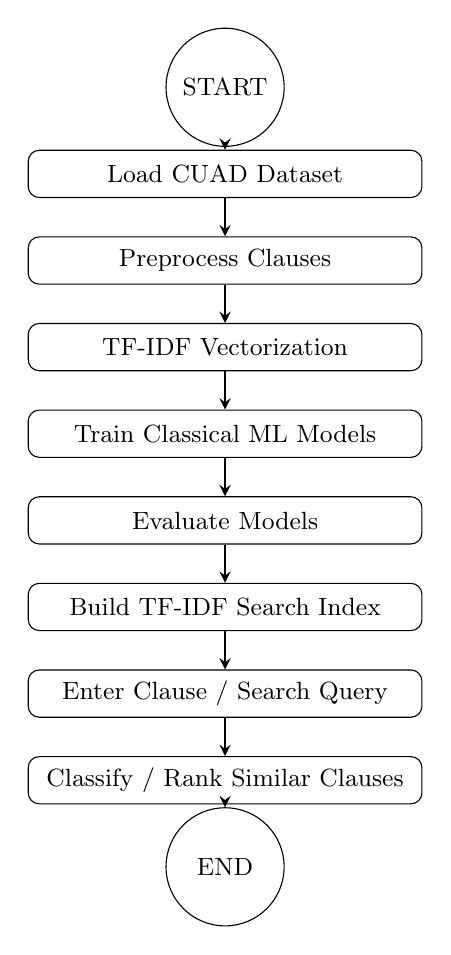
\begin{tikzpicture}[
  node distance=1.1cm,
  every node/.style={fill=white, draw=black, rounded corners, font=\small, minimum width=5cm, minimum height=0.6cm, align=center},
  arrow/.style={thick, ->, >=stealth}
]
  \node (start) [circle, draw, minimum width=1.5cm] {START};
  \node (load) [below of=start] {Load CUAD Dataset};
  \node (preprocess) [below of=load] {Preprocess Clauses};
  \node (vectorize) [below of=preprocess] {TF-IDF Vectorization};
  \node (train) [below of=vectorize] {Train Classical ML Models};
  \node (evaluate) [below of=train] {Evaluate Models};
  \node (build) [below of=evaluate] {Build TF-IDF Search Index};
  \node (query) [below of=build] {Enter Clause / Search Query};
  \node (classify) [below of=query] {Classify / Rank Similar Clauses};
  \node (end) [below of=classify, circle, draw, minimum width=1.5cm] {END};

  \draw [arrow] (start) -- (load);
  \draw [arrow] (load) -- (preprocess);
  \draw [arrow] (preprocess) -- (vectorize);
  \draw [arrow] (vectorize) -- (train);
  \draw [arrow] (train) -- (evaluate);
  \draw [arrow] (evaluate) -- (build);
  \draw [arrow] (build) -- (query);
  \draw [arrow] (query) -- (classify);
  \draw [arrow] (classify) -- (end);
\end{tikzpicture}
\caption{Activity diagram: TF-IDF + classical ML clause classification and search pipeline}
\label{fig:activity_diagram}
\end{figure}

\newpage

\section{Project Pipeline}

\subsection{Project Pipeline Diagram with Explanation}
\begin{figure}[h]
\centering
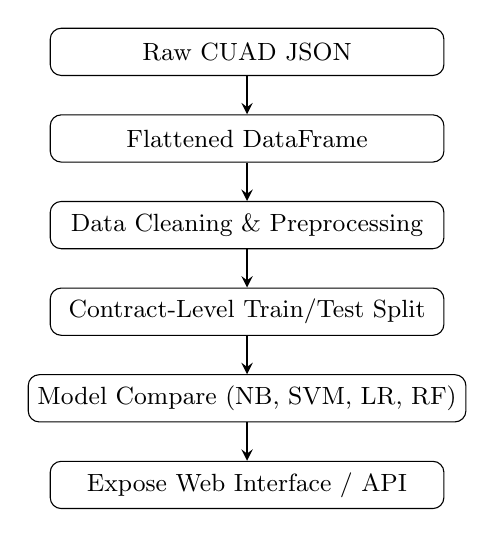
\begin{tikzpicture}[
  node distance=1.1cm,
  every node/.style={fill=white, draw=black, rounded corners, font=\small, minimum width=5cm, minimum height=0.6cm, align=center},
  arrow/.style={thick, ->, >=stealth}
]
  \node (raw) {Raw CUAD JSON};
  \node (flatten) [below of=raw] {Flattened DataFrame};
  \node (clean) [below of=flatten] {Data Cleaning \& Preprocessing};
  \node (split) [below of=clean] {Contract-Level Train/Test Split};
  \node (train) [below of=split] {Model Compare (NB, SVM, LR, RF)};
  \node (api) [below of=train] {Expose Web Interface / API};

  \draw [arrow] (raw) -- (flatten);
  \draw [arrow] (flatten) -- (clean);
  \draw [arrow] (clean) -- (split);
  \draw [arrow] (split) -- (train);
  \draw [arrow] (train) -- (api);
\end{tikzpicture}
\caption{ClauseIQ project pipeline flow}
\label{fig:project_pipeline}
\end{figure}

\paragraph{Data}
The pipeline begins with the CUAD dataset (510 contracts, 41 clause categories), which is flattened from its SQuAD-style JSON format into a clause-level table as described in Section \ref{ch:system_analysis}. Exploratory data analysis (class distribution, length distribution, missing-value and duplicate checks) is performed to understand the corpus, followed by data cleaning and TF-IDF-based preprocessing as described in Section \ref{subsec:data_cleaning}.

\paragraph{Model Building}
The cleaned, vectorised dataset is split into stratified training (80\%) and testing (20\%) subsets. Four classical ML models — Multinomial Naive Bayes, Linear SVM, Logistic Regression and Random Forest — are trained on the TF-IDF features with class-weighting to address the imbalance documented in Section \ref{subsec:class_analysis}, and compared using macro-F1, per-class F1 and accuracy to select the best-performing classifier.

\paragraph{Intelligent Search \& Deployment}
Independently of classification, a TF-IDF index of the full clause corpus is built to support cosine-similarity-based intelligent search: a free-text query is vectorised in the same TF-IDF space and the most similar clauses are ranked and returned. The selected classifier and the search index are planned to be persisted (via joblib) and exposed through a simple web/API interface so a user can classify a new clause or search the corpus for clauses matching a natural-language query.

\section{System Implementation}
\label{sec:system_implementation}
This section documents the Python implementation details for the various preprocessing, feature extraction, classifier training, and cosine similarity search modules of ClauseIQ.

\subsection{Text Preprocessing and Data Cleaning}
To normalize raw contract texts, whitespace is collapsed and non-standard characters are removed, retaining common punctuation marks. Short clause spans with fewer than 3 words are filtered out to improve classification quality.
\begin{lstlisting}[language=Python, caption={Text Cleaning and Normalization Code Snippet}]
import re

def clean_text(t):
    t = re.sub(r'\s+', ' ', str(t))                  # collapse whitespace
    t = re.sub(r"[^A-Za-z0-9.,;:()%$\-\s]", ' ', t)  # strip odd artefacts
    return t.strip()

df['clean_text'] = df['clause_text'].apply(clean_text)
df_clean = df[df['clean_text'].str.split().str.len() >= 3]
\end{lstlisting}

\subsection{TF-IDF Feature Extraction}
Cleaned contract clauses are vectorized into a high-dimensional, length-normalized feature space using unigram and bigram representation, with the vocabulary capped at the top 5,000 terms.
\begin{lstlisting}[language=Python, caption={TF-IDF Feature Extraction Code Snippet}]
from sklearn.feature_extraction.text import TfidfVectorizer

tfidf = TfidfVectorizer(max_features=5000, stop_words='english',
                        ngram_range=(1,2), min_df=2)
X = tfidf.fit_transform(df_clean['clean_text'])
\end{lstlisting}

\subsection{Pipeline Training and Search Workflows}
The classifier is trained using a stratified split to ensure full class representation. The search module uses the same TF-IDF space and Cosine Similarity to compute ranking scores for user queries.
\begin{lstlisting}[language=Python, caption={Pipeline Training and Inference Pseudocode}]
# TF-IDF + Classifier Training and Similarity Searching

def train_clause_classifier(D, model_type):
    # D: Clause dataset with text X and labels Y
    X_clean = clean_text(D.text)
    tfidf = fit_tfidf(X_clean, max_features=5000, ngram_range=(1,2))
    X_train, X_test, y_train, y_test = stratified_split(tfidf, D.category, test_size=0.2)
    model = init_model(model_type, class_weight='balanced')   # NB / SVM / LR / RF
    model.fit(X_train, y_train)
    y_pred = model.predict(X_test)
    metrics = evaluate(y_test, y_pred)   # macro-F1, per-class F1, accuracy
    return model, tfidf, metrics

def search_clauses(query, corpus_vectors, tfidf, top_k):
    q_vec = tfidf.transform([query])
    scores = cosine_similarity(q_vec, corpus_vectors)
    return top_k_ranked(scores, top_k)
\end{lstlisting}

\section{Feasibility Analysis}
Feasibility has been assessed across technical, economic and operational dimensions, consistent with the scope-controlled, classical-ML approach agreed with the project guide.

\subsection{Technical Feasibility}
\begin{itemize}
    \item \textbf{Data processing:} CUAD is a public, well-documented, CC-BY-4.0-licensed dataset; it was downloaded directly from the official GitHub repository and successfully flattened into a clean, tabular clause dataset (13,823 rows) using standard Python libraries (\texttt{pandas}, \texttt{json}, \texttt{re}), confirming that data acquisition and preprocessing are fully achievable within the project's technical resources.
    \item \textbf{Machine learning:} TF-IDF vectorisation and the four chosen classifiers (Naive Bayes, SVM, Logistic Regression, Random Forest) are all implemented in \texttt{scikit-learn}, a mature, well-documented, free library; no custom low-level ML code or GPU hardware is required.
    \item \textbf{Search module:} cosine similarity over TF-IDF vectors uses the same \texttt{scikit-learn} feature space already built for classification, so no additional infrastructure (e.g. a dedicated vector database) is required at this project's scale (13,823 clauses).
    \item \textbf{Deployment:} the trained classifier and TF-IDF index can be serialized with \texttt{joblib} and served through a lightweight Python web framework (e.g. FastAPI), consistent with tooling already used elsewhere in the department's mini projects.
\end{itemize}

\subsection{Economic Feasibility}
All software used — Python, pandas, scikit-learn, matplotlib/seaborn, Flask/FastAPI, joblib — is free and open-source; the CUAD dataset itself is free and openly licensed (CC BY 4.0).
No paid annotation, cloud GPU, or third-party API costs are required for the classical ML approach adopted here, keeping the project's running cost close to zero beyond standard computer hardware and development time.
The resulting tool has clear practical value — faster clause triage for legal/compliance teams, students, and paralegals reviewing standard commercial contracts — which justifies the (minimal) development effort.

\subsection{Operational Feasibility}
End users (e.g. a paralegal or contract reviewer) only need to paste clause text or a search query into a simple web interface; no legal-technology or machine-learning expertise is required to operate the system.
Because the underlying models are lightweight classical classifiers rather than large neural networks, inference is fast enough for interactive, single-clause or single-query use on ordinary hardware, without needing a GPU or specialised serving infrastructure.
The system's scope is intentionally bounded to the 41 CUAD categories and to classical ML, which keeps the operational surface small and maintainable within a single-semester mini project timeline, while leaving a clear, well-justified extension path (transformer / RAG-based deep learning) for a future main project.

\newpage

% ==========================================
% REFERENCES
% ==========================================
\begin{thebibliography}{99}

\bibitem{legalreasoner}
Quevedo Caballero E., Černý T., Rodriguez A., Rivas P., Yero J., Sooksatra K., Taibi D.,
``Legal Natural Language Processing From 2015 to 2022: A Comprehensive Systematic Mapping Study of Advances and Applications,''
\textit{IEEE Access}, vol. 12, pp. 145286--145317, 2024.
\url{https://doi.org/10.1109/ACCESS.2024.3414967}

\bibitem{siino2025}
Siino M., Falco M., Croce D., Rosso P.,
``Exploring LLMs Applications in Law: A Literature Review on Current Legal NLP Approaches,''
\textit{IEEE Access}, vol. 13, pp. 18253--18276, 2025.
\url{https://doi.org/10.1109/ACCESS.2025.3533217}

\bibitem{hasib2023}
Kutbi M.,
``Named Entity Recognition Utilized to Enhance Text Classification While Preserving Privacy,''
\textit{IEEE Access}, vol. 11, pp. 117576--117581, 2023.
\url{https://doi.org/10.1109/ACCESS.2023.3325895}

\bibitem{cuad}
D. Hendrycks, C. Burns, A. Chen, and S. Ball,
``CUAD: An Expert-Annotated NLP Dataset for Legal Contract Review,''
\textit{Proceedings of the Neural Information Processing Systems (NeurIPS)}, 2021.
\url{https://arxiv.org/abs/2103.06268}

\bibitem{scikit-learn}
F. Pedregosa et al.,
``Scikit-learn: Machine Learning in Python,''
\textit{Journal of Machine Learning Research}, vol. 12, pp. 2825--2830, 2011.

\bibitem{spacy}
M. Honnibal and I. Montani,
``spaCy: Industrial-strength Natural Language Processing in Python,''
\textit{Zenodo}, 2017.

\end{thebibliography}

\end{document}
